\documentclass[12pt,a4paper]{article}
\usepackage[utf8]{vietnam}
\usepackage{amsmath}
\usepackage{amsfonts}
\usepackage{amssymb}
\usepackage{caption}
\usepackage{subcaption}
\usepackage{graphicx}
\title{Drones In Trees}
\author{Group 1 - BBLAB}
\date{February 2023}
\begin{document}
\maketitle
\begin{abstract}
    Việc bảo vệ và phục hồi môi trường là việc rất quan trong nó liên quan đến sự sống của mọi loài trên trái đất, nhưng sự khan hiếm dữ liệu về tình trạng và sự phân bố đa dạng sinh học khiến những nỗ lực gặp rủi ro. DNA do các sinh vật phóng thích vào môi trường hay DNA môi trường (eDNA), có thể được sử dụng để giám sát đa dạng sinh học theo cách có thể mở rộng nếu được trang bị công cụ thích hợp. Máy bay không người lái là sự lựa chọn thích hợp cho công việc này, kết hợp lồng cảm ứng lực với chiến lược điều khiển dựa trên xúc giác để thiết lập và duy trì liên lạc với bề mặt của cành cây. Sau đó, eDNA được thu thập bằng cách sử dụng một mặt kết dính được tích hợp trong lồng của máy bay. Việc kết hợp robot với lấy mẫu eDNA từ nhiều loại chất nền trên mặt đất không thể đưa ra giải pháp giám sát đa dạng sinh học trên diện rộng.
\end{abstract}
\tableofcontents
\newpage
\section{Giới Thiệu}
Đa dạng sinh thái đang suy giảm nhanh chóng với ước tính khoảng 1 triệu loài bị đe dọa tuyệt chủng trong hai thập kỉ tới. Do vậy, bảo tồn sinh thái là rất quan trọng và cấp bách. Điều đó, phụ thuộc vào việc thu thập dữ liệu chính xác về sự phân bố của loài và quy mô quần thể trên các quy mô sinh thái đó. Các cuộc khảo sát DNA môi trường (eDNA) gần đây đã thu hút được sự quan tâm trên toàn thế giới đối với việc giám sát đa dạng sinh học. Các khảo sát mã hóa siêu dữ liệu eDNA có thể đồng thời phát hiện nhiều loài từ cả ba lĩnh vực sống từ một mẫu duy nhất mà không có bất kỳ dấu hiệu rõ ràng nào về sự hiện diện của chúng, các phương pháp tự động, cơ giới hóa để thu thập dấu vết DNA có khả năng tạo thuận lợi cho việc khảo sát đa dạng sinh học trên quy mô không gian lớn.\\
\linebreak
Robot trên không được trang bị máy ảnh hoặc máy theo dõi tần số cao đã hỗ trợ thành công việc giám sát động vật hoang dã  và tính linh hoạt của chúng cũng có thể điều chỉnh để thu thập các mẫu eDNA. Việc thu thập thủ công các môi trường liên quan vẫn là một nút thắt trong việc mở rộng các cuộc điều tra eDNA đặc biệt là trong các hệ sinh thái trên cạn. Tán rừng đại diện cho một môi trường sống quan trọng đối với đa dạng sinh học, mà nhìn chung vẫn chưa được khảo sát đầy đủ. Việc sử dụng robot để khảo sát eDNA từ những địa điểm như vậy cho phép chúng ta cải thiện được môi trường sống. việc khảo sát eDNA bằng máy bay không người lái trong rừng đặt ra những thách thức khoa học mở trong cả lĩnh vực robot và sinh học.\\
\linebreak
Yêu cầu chạm vào các cành cây để thu thập eDNA chuyển thành nhu cầu cho máy bay không người lái thiết lập liên lạc với môi trường xung quanh bằng cách tác dụng lực lên các bề mặt. Kiểm tra dựa trên tiếp xúc và thao tác trên không, thường chỉ giới hạn ở các kết cấu có bề mặt cứng. Tuy nhiên, các nhánh là một chất nền không tĩnh điện mà độ tuân thủ của nó có thể thay đổi tới bốn bậc độ lớn. Đối với các phương pháp tương tác vật lý hiện tại, phản ứng đàn hồi chưa biết của các nhánh, cũng như sự sai lệch trong quá trình tiếp cận gây ra bởi các dao động không thể đoán trước của nhánh, có thể khiến máy bay không người lái mất ổn định, bị lật hoặc bị ném ra xa. Hơn nữa, robot có thể thu thập eDNA, chẳng hạn như từ bề mặt, nhưng điều này chưa được thử nghiệm rộng rãi trên bề mặt cây. eDrone sử dụng chiến lược tương tác này để thiết lập và duy trì tiếp xúc trên bề mặt trên của các nhánh, nơi eDNA được thu thập bởi một bề mặt dính được tích hợp trong lồng.\\
\newpage
\begin{figure}
    \centering
    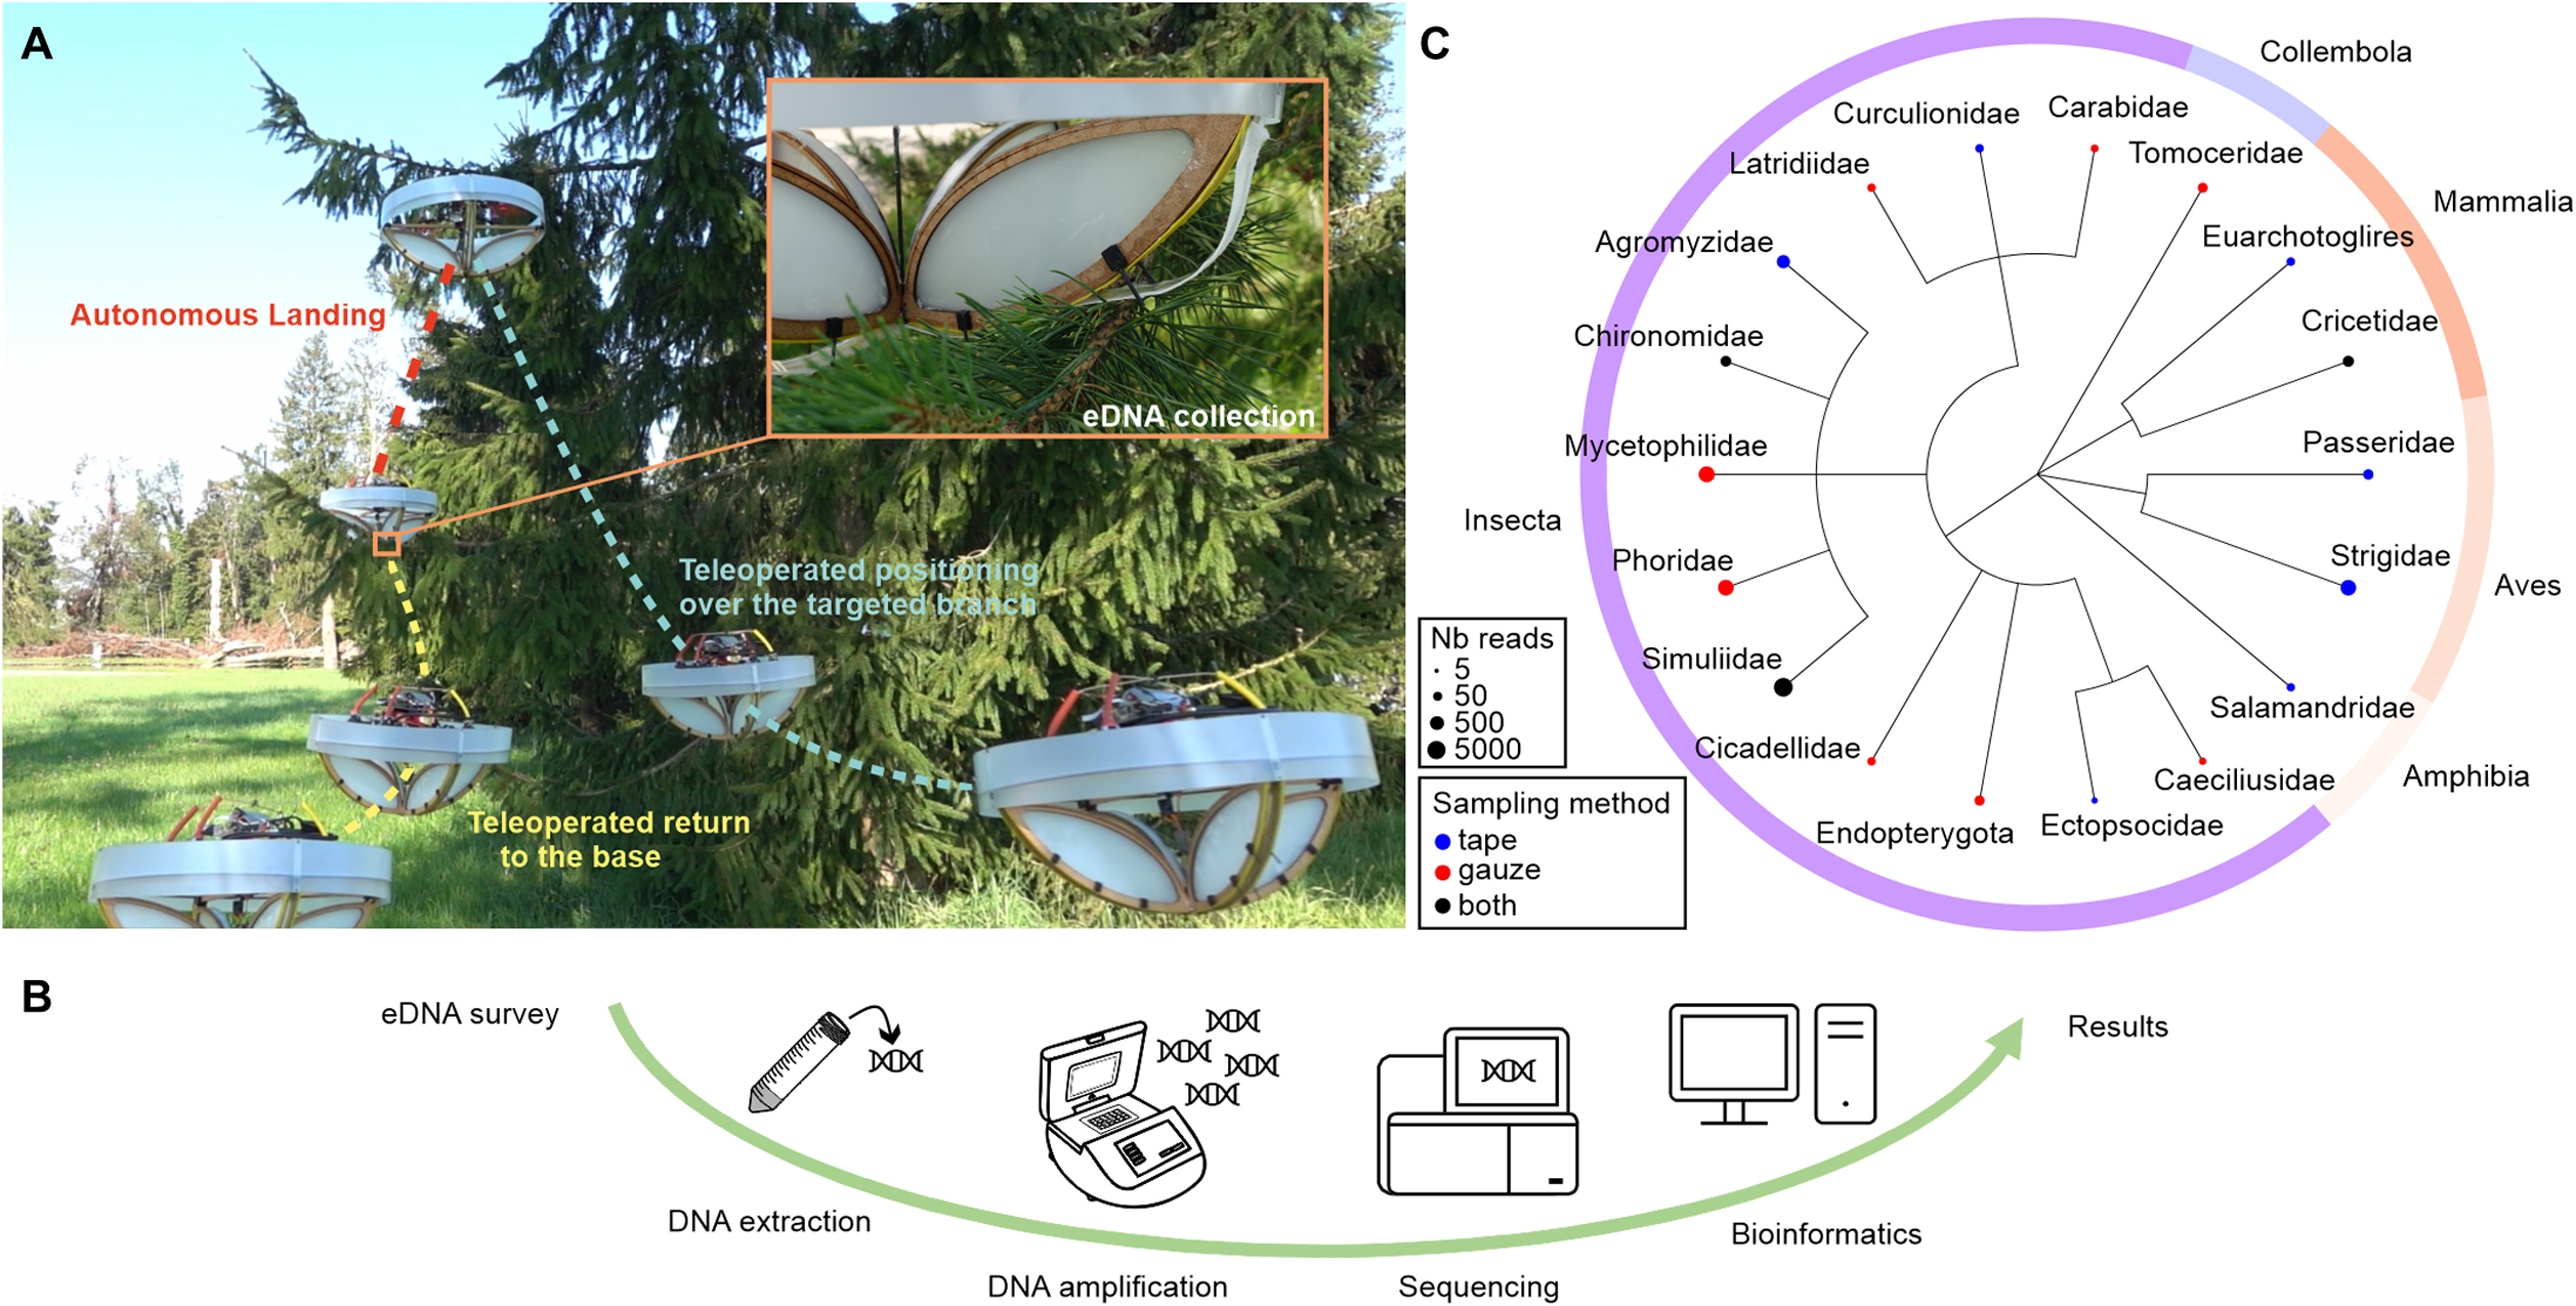
\includegraphics[scale = 0.7]{hinh 1}
    \caption{\textit{Sơ đồ khảo sát đa dạng sinh học với máy bay không người lái thu thập eDNA.}}
    \label{fig1}
\end{figure} 
\section{Khái Niệm Và Cơ Sở Thiết Kế Robot}
\subsection{Khái Niệm}
Máy bay không người lái được phát triển để tương tác vật lý với các nhánh tuân thủ. eDrone được thiết kế để tối đa hóa khả năng chống sai lệch khi hạ cánh trên các cành cây bằng cách có thể cảm nhận và xử lý các điểm tiếp xúc đơn lẻ từ nhiều hướng khác nhau và trên diện tích bề mặt lớn. Điều này đạt được bằng cách tích hợp máy bay không người lái vào một bộ phận kết thúc hình bán cầu với cảm nhận lực phân tán, đồng thời đóng vai trò là bộ phận hạ cánh và lồng bảo vệ. 
\subsection{Cơ Sở Thiết Kế Robot}
Drones bao gồm một quadcopter được trang bị lồng cảm ứng lực tích hợp bộ thu eDNA để lấy eDNA bề mặt từ các nhánh cây. Bản chất tuân thủ của chất nền này dẫn đến những thách thức trong thiết kế bộ tạo đầu cuối chạm vào nhánh, chiến lược cảm nhận lực và cơ chế thu thập eDNA dựa trên cảm ứng bề mặt. Máy bay không người lái tương tác với các cấu trúc cứng nhắc ưu tiên bộ tạo đầu cuối một điểm để định vị lực tương tác trong khu vực được nhắm mục tiêu, trong khi hạ cánh trên các nhánh linh hoạt, không tĩnh điện đòi hỏi sự chắc chắn đối với các sai lệch tuyến tính và góc chắc chắn phát sinh từ các chuyển động không thể đoán trước của các nhánh.\\
\linebreak
Máy bay không người lái có thể chạm vào các nhánh dọc theo mỗi cung, cho phép tương tác đa hướng và độ bền đối với các sai lệch tuyến tính . Đường kính của lồng là kết quả của sự đánh đổi giữa các yêu cầu trái ngược nhau. Một mặt, một chiếc lồng lớn chịu được độ lệch lớn hơn và khoảng cách giữa máy bay không người lái xa hơn với thảm thực vật, giảm nguy cơ cành cây hoặc lá cây mắc vào cánh quạt. Mặt khác, một chiếc lồng có diện tích nhỏ giúp máy bay không người lái phù hợp hơn để bay trong môi trường lộn xộn và giảm thời điểm mất ổn định do lực tương tác với nhánh gây ra.\\
\linebreak
Chiến lược cảm biến lực dựa trên một cảm biến tải trọng sáu trục, kết nối bộ tạo kết thúc có lồng với khung của robot trên không. Mặc dù được tập trung hóa hệ thống cảm biến xúc giác này cung cấp nhận thức phân tán bằng cách đo lực tương tác tại điểm tiếp xúc, lực này có thể xảy ra ở bất kỳ đâu dọc theo bốn cung của lồng. Mỗi vòng cung của lồng chứa một cơ chế thu thập eDNA. Kết quả của cơ sở thiết kế này là một robot bay trên không nặng 1,2 kg với dấu chân hình tròn có đường kính 440 mm. Thông tin chi tiết khác về thiết kế cơ khí và thiết bị điện tử cho chuyến bay tự động và điều khiển từ xa có sẵn trong vật liệu và phương pháp.\\
\begin{figure}
    \centering
    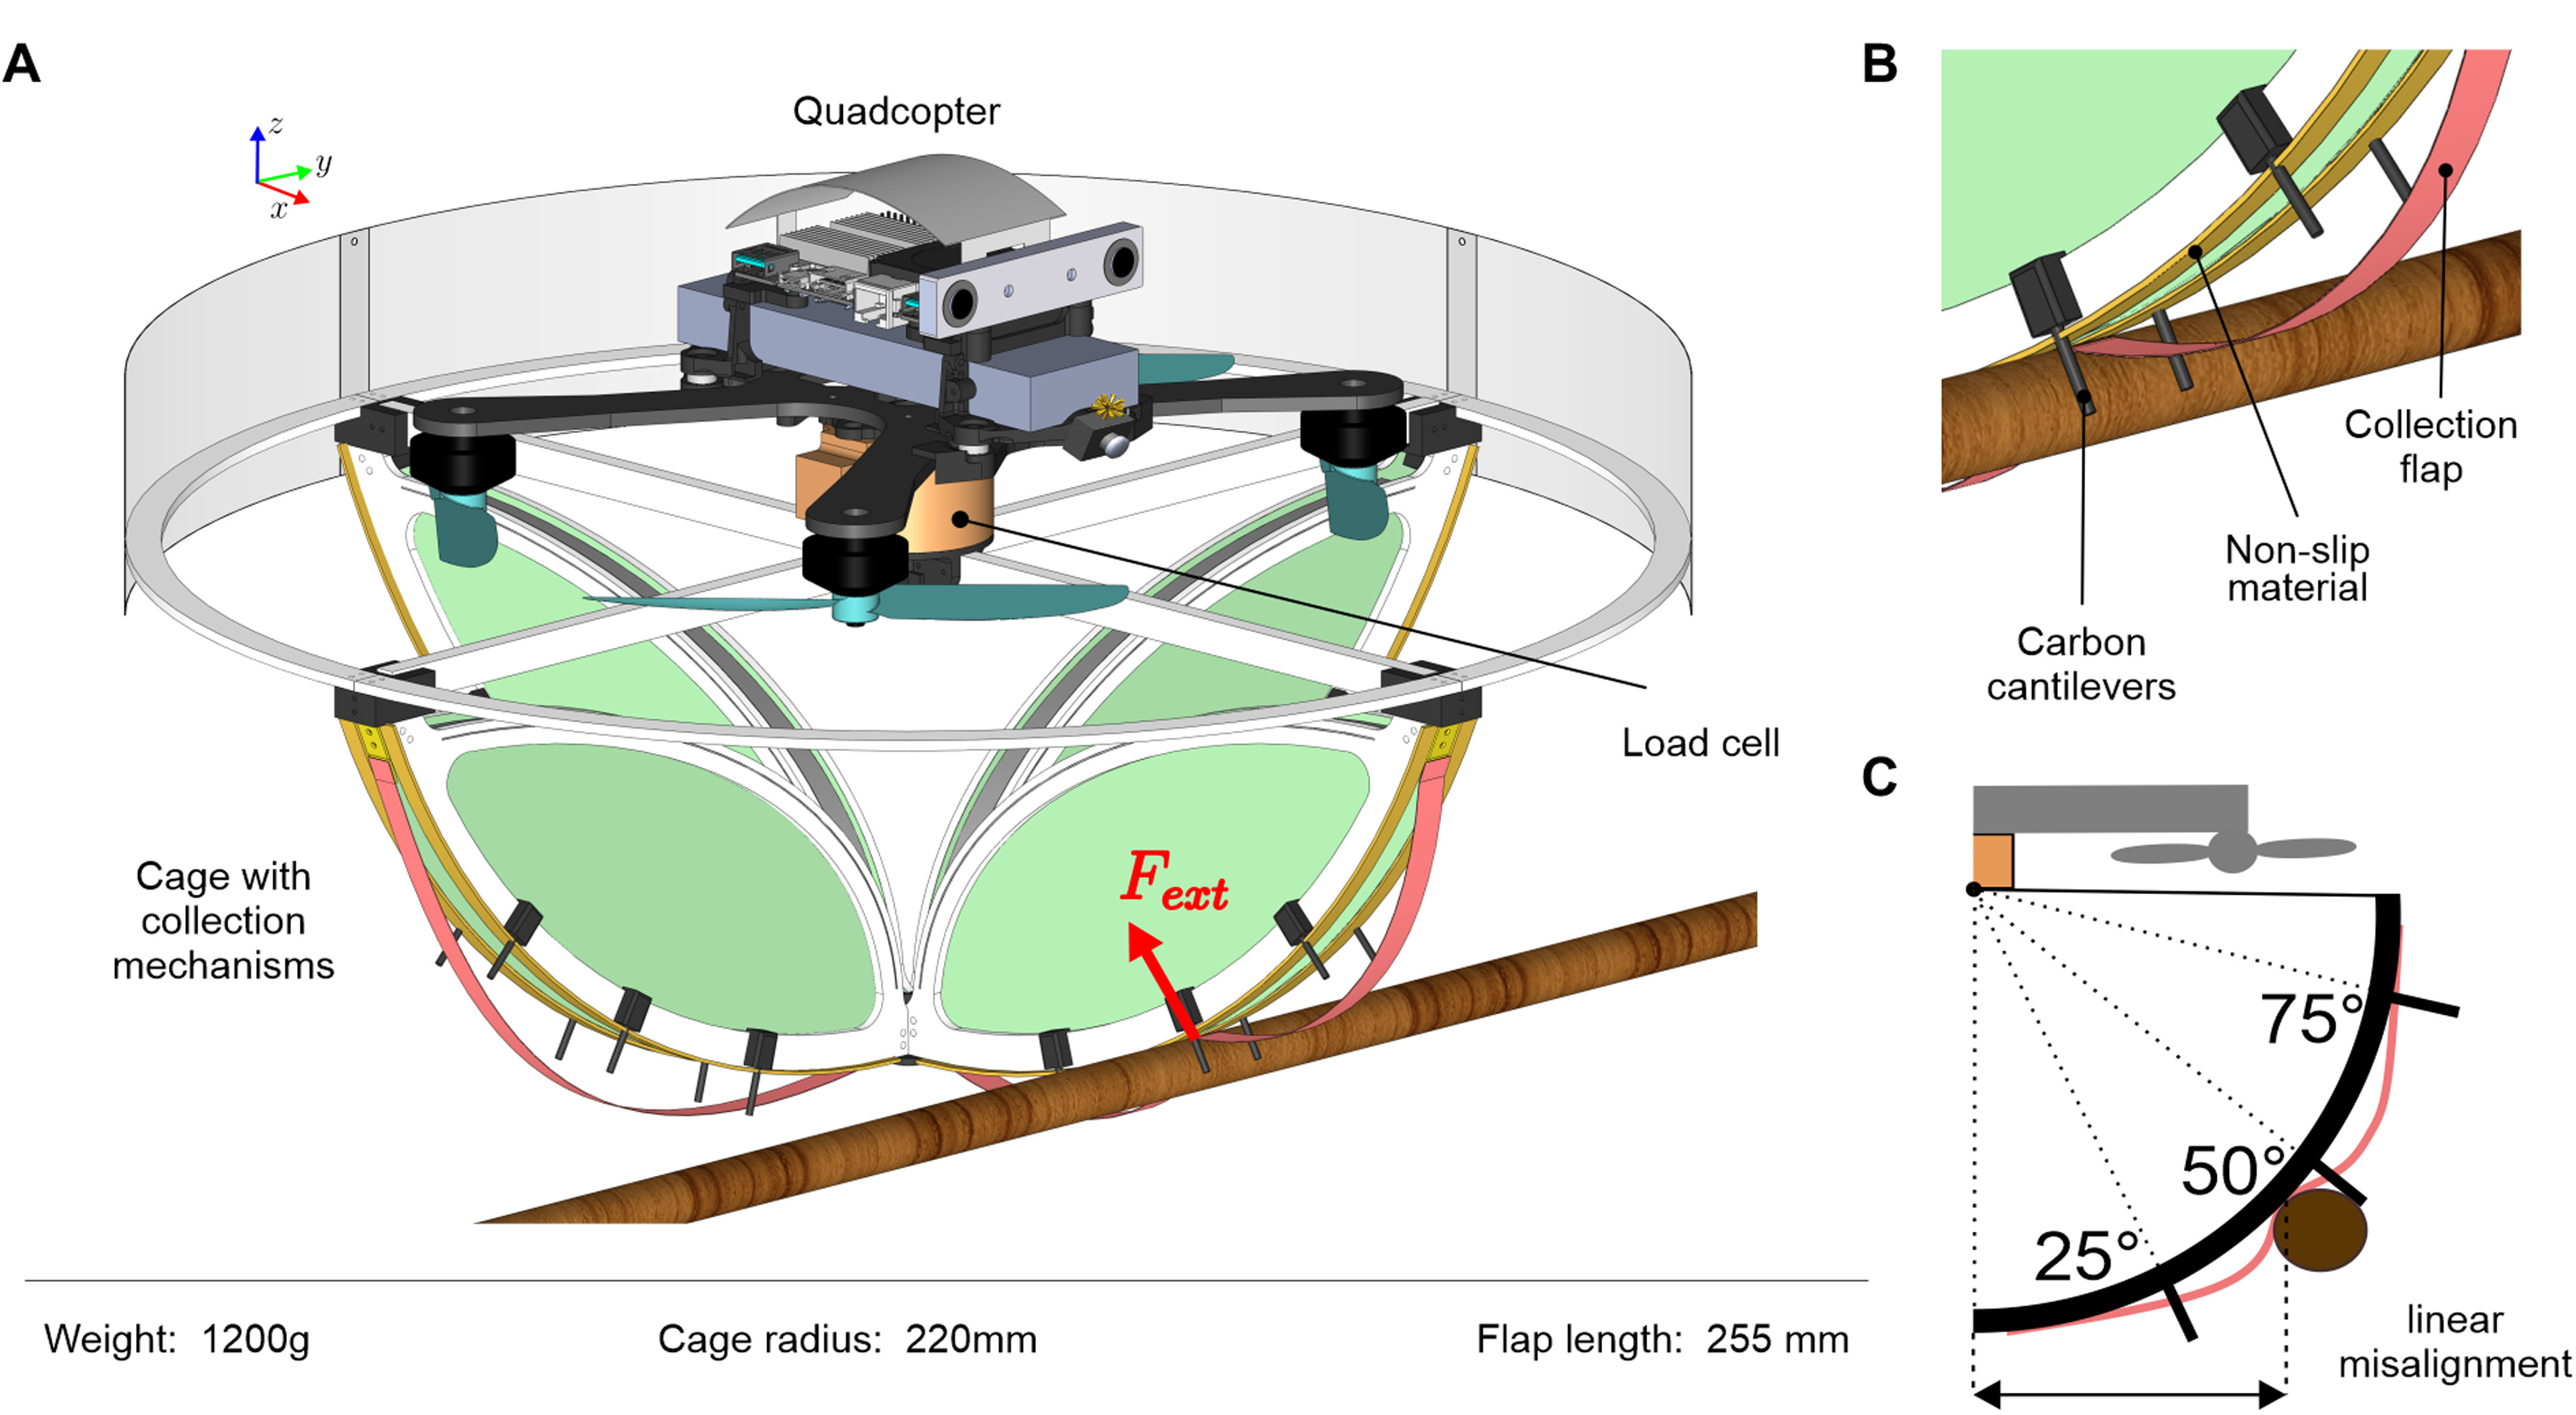
\includegraphics[scale = 0.9]{hinh 2}
    \caption{\textit{Kiến trúc eDrone.}}
    \label{fig2}
\end{figure}
\subsection{Cơ Sở Chiến Lược Hạ Cánh}
Drones hạ cánh và duy trì liên lạc với các nhánh để thu thập eDNA. Sự tương tác này trở nên khó khăn vì máy bay không người lái không biết độ cứng (K) của các nhánh. Để phát triển chiến lược hạ cánh, chúng tôi đã nghiên cứu trạng thái cân bằng phẳng của eDrone trên một thanh xà có bản lề uốn. Mô hình cho thấy rằng độ nghiêng là cần thiết ngay cả đối với các dầm cứng và tăng lên đối với các giá trị độ nghiêng và độ tuân thủ ban đầu cao hơn. Phải tránh tình trạng này vì chiến lược kiểm soát dựa trên xúc giác được chính thức hóa để xử lý một điểm tiếp xúc duy nhất trên các vòng cung của lồng.\\
\begin{figure}[ht!]
    \centering
    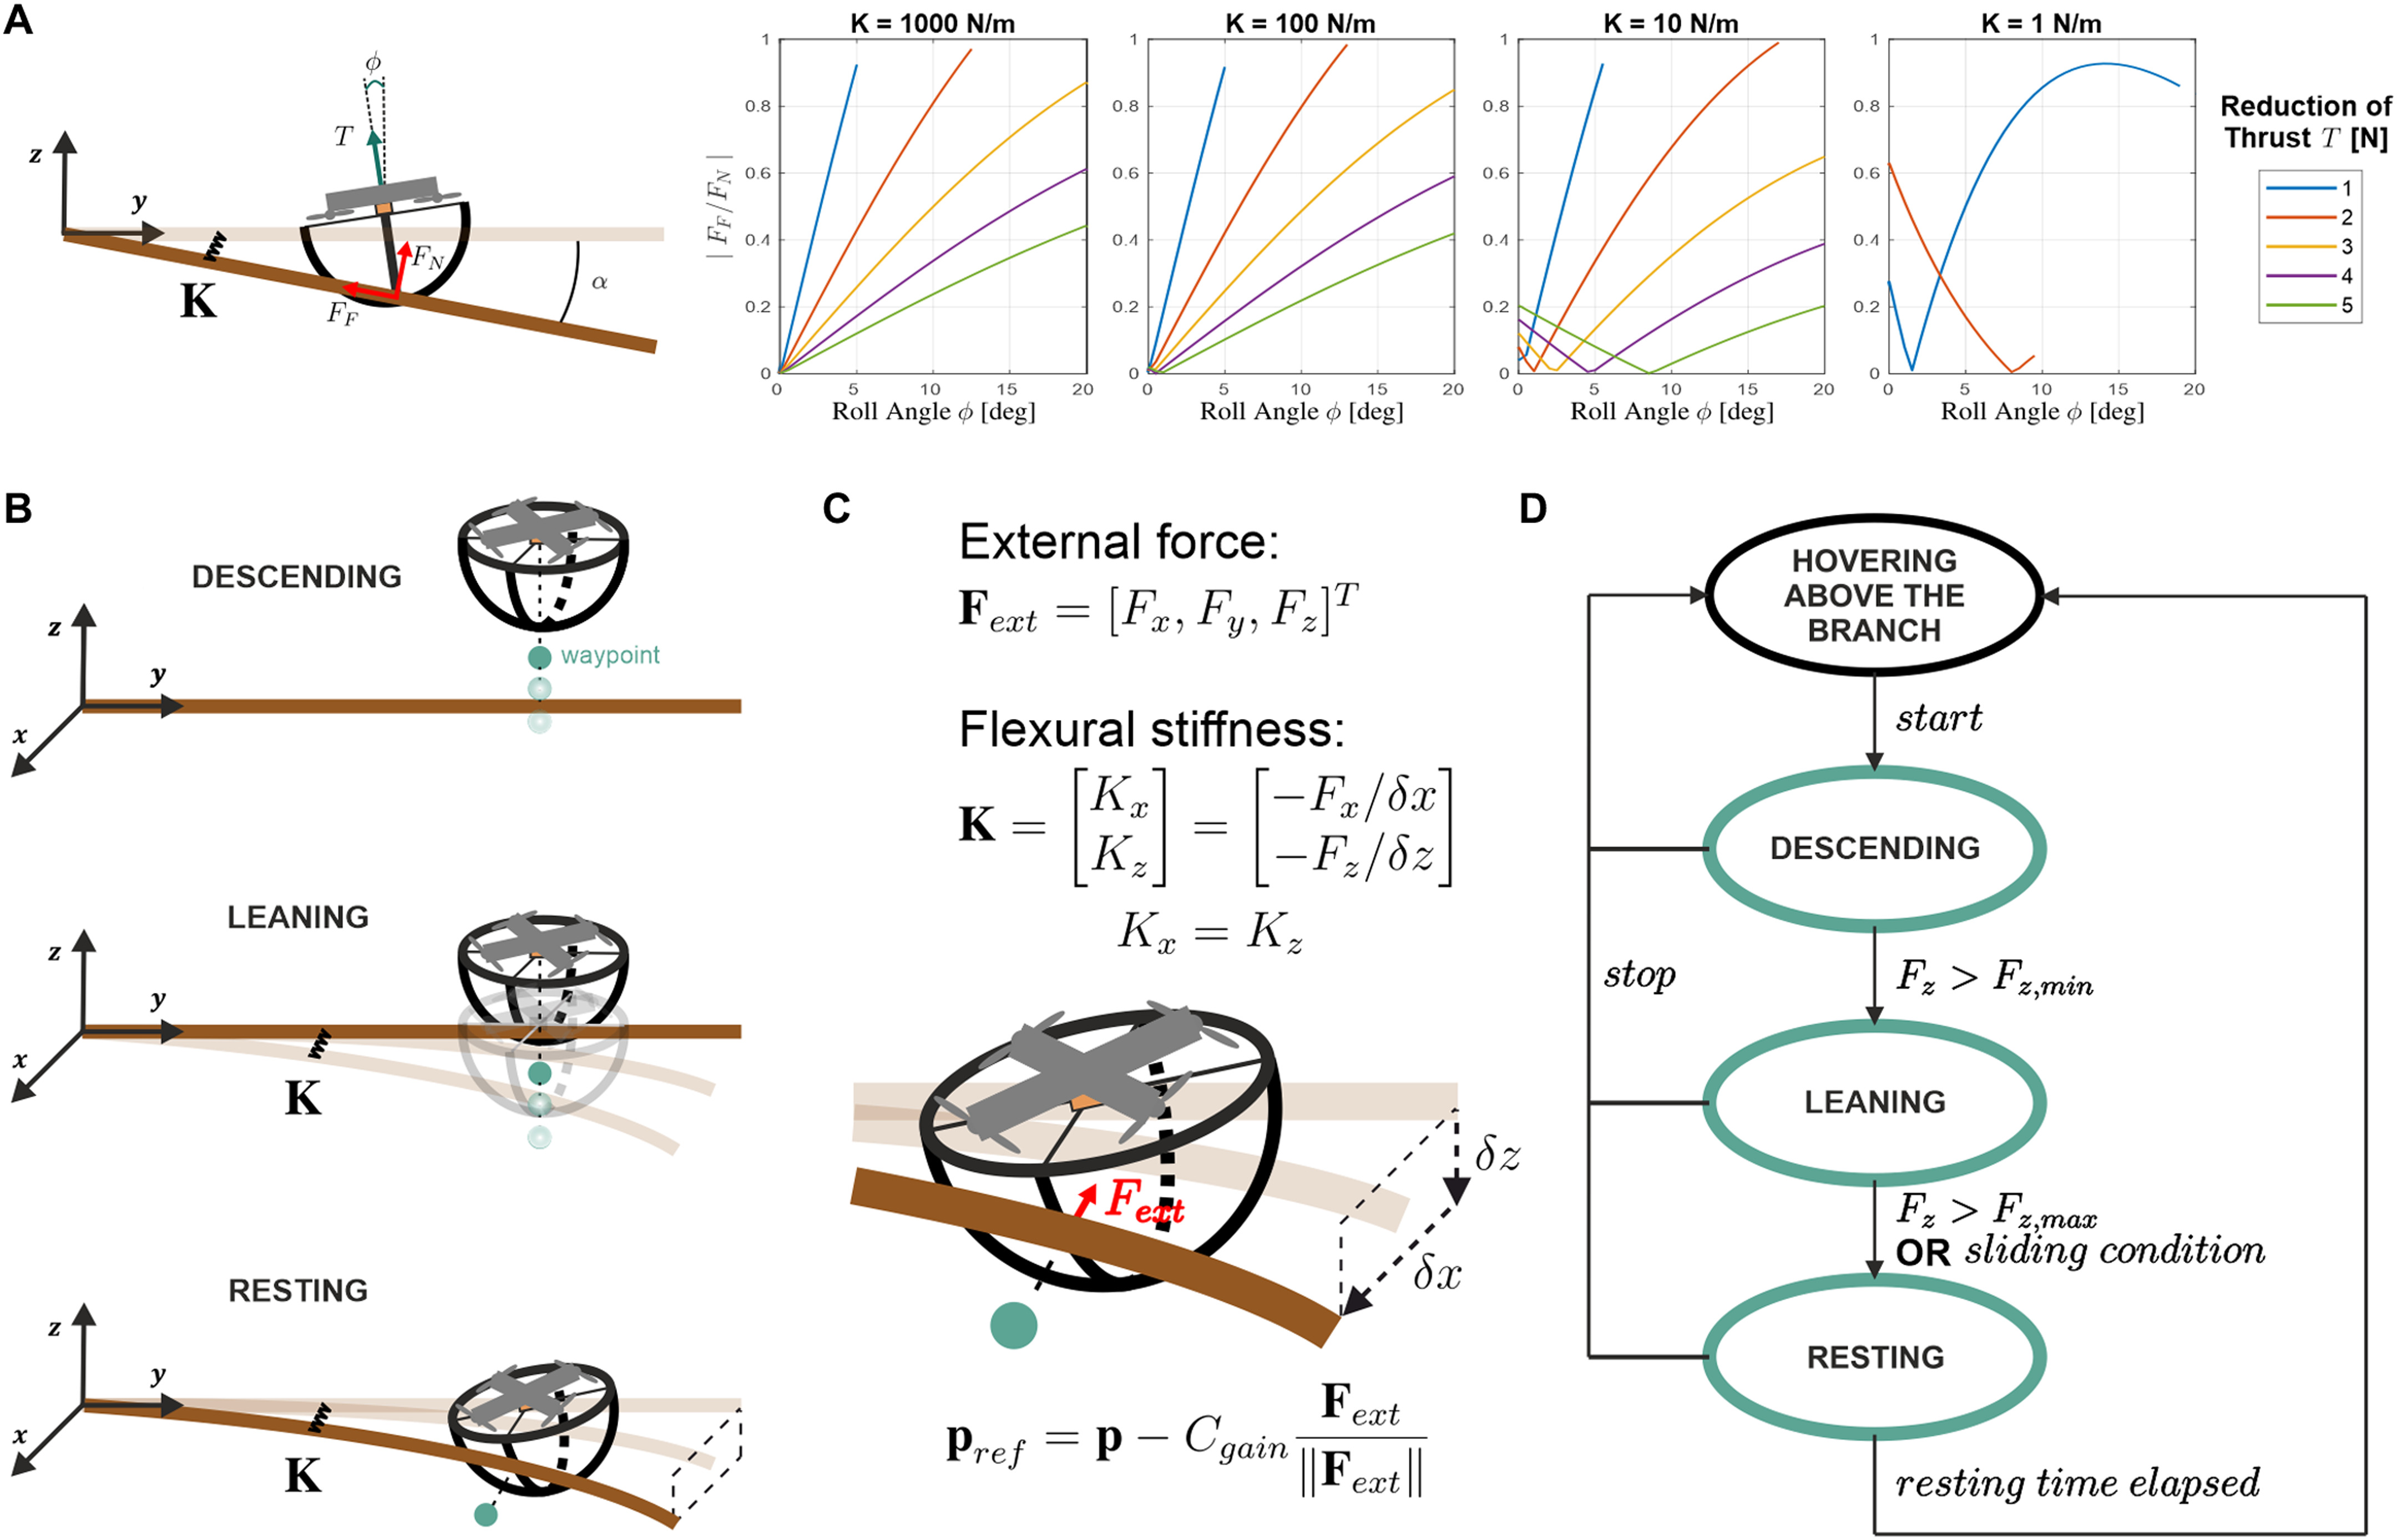
\includegraphics[scale = 0.7]{hinh 3}
    \caption{\textit{Chiến lược hạ cánh}}
    \label{fig3}
\end{figure} \\
Đầu tiên, máy bay không người lái được điều khiển từ xa phía trên một nhánh và được thả ở trạng thái lơ lửng. Do đó, nó tự động đi xuống theo quỹ đạo tham chiếu bao gồm các điểm tham chiếu thẳng đứng cho đến khi lồng cảm biến lực phát hiện hợp đồng với nhánh (giảm dần). Ngưỡng này phải được đặt cao hơn độ ồn của cảm biến tải trọng để tránh phát hiện tiếp xúc sai trong điều kiện bay tự do (trong trường hợp của chúng tôi, ngưỡng được đặt thành 0,35 N).\\
\\
Sau khi phát hiện tiếp xúc, HWR tiếp tục ra lệnh cho máy bay không người lái cúi xuống thông qua các điểm tham chiếu thẳng đứng, giảm lực đẩy và tiếp tục đo lực tương tác. Trong giai đoạn này, HWR giám sát các điều kiện nguy hiểm tiềm tàng, chẳng hạn như lật hoặc trượt khỏi cành cây, điều này sẽ khiến máy bay không người lái thực hiện thao tác lảng tránh và quay trở lại trạng thái lơ lửng. Điều này, được gọi là “điều kiện trượt” trong lưu đồ, được thực hiện bằng cách theo dõi các thay đổi giữa vị trí hiện tại của máy bay không người lái và vị trí của nó trong lần tiếp xúc đầu tiên với chi nhánh. Điều này đảm bảo rằng máy bay không người lái vẫn nằm trong phạm vi hoạt động an toàn, vì nhánh không bị uốn cong quá nhiều, tránh va chạm với vòng ngang của lồng và giảm thiểu nguy cơ trượt đối với góc nghiêng thấp, lực đẩy được giữ gần với giá trị lơ lửng, do đó cho phép thực hiện các thao tác lảng tránh nhanh hơn.\\
\subsection{Xác Thực Thử Nghiệm HWR}
\begin{figure}[ht!]
    \centering
    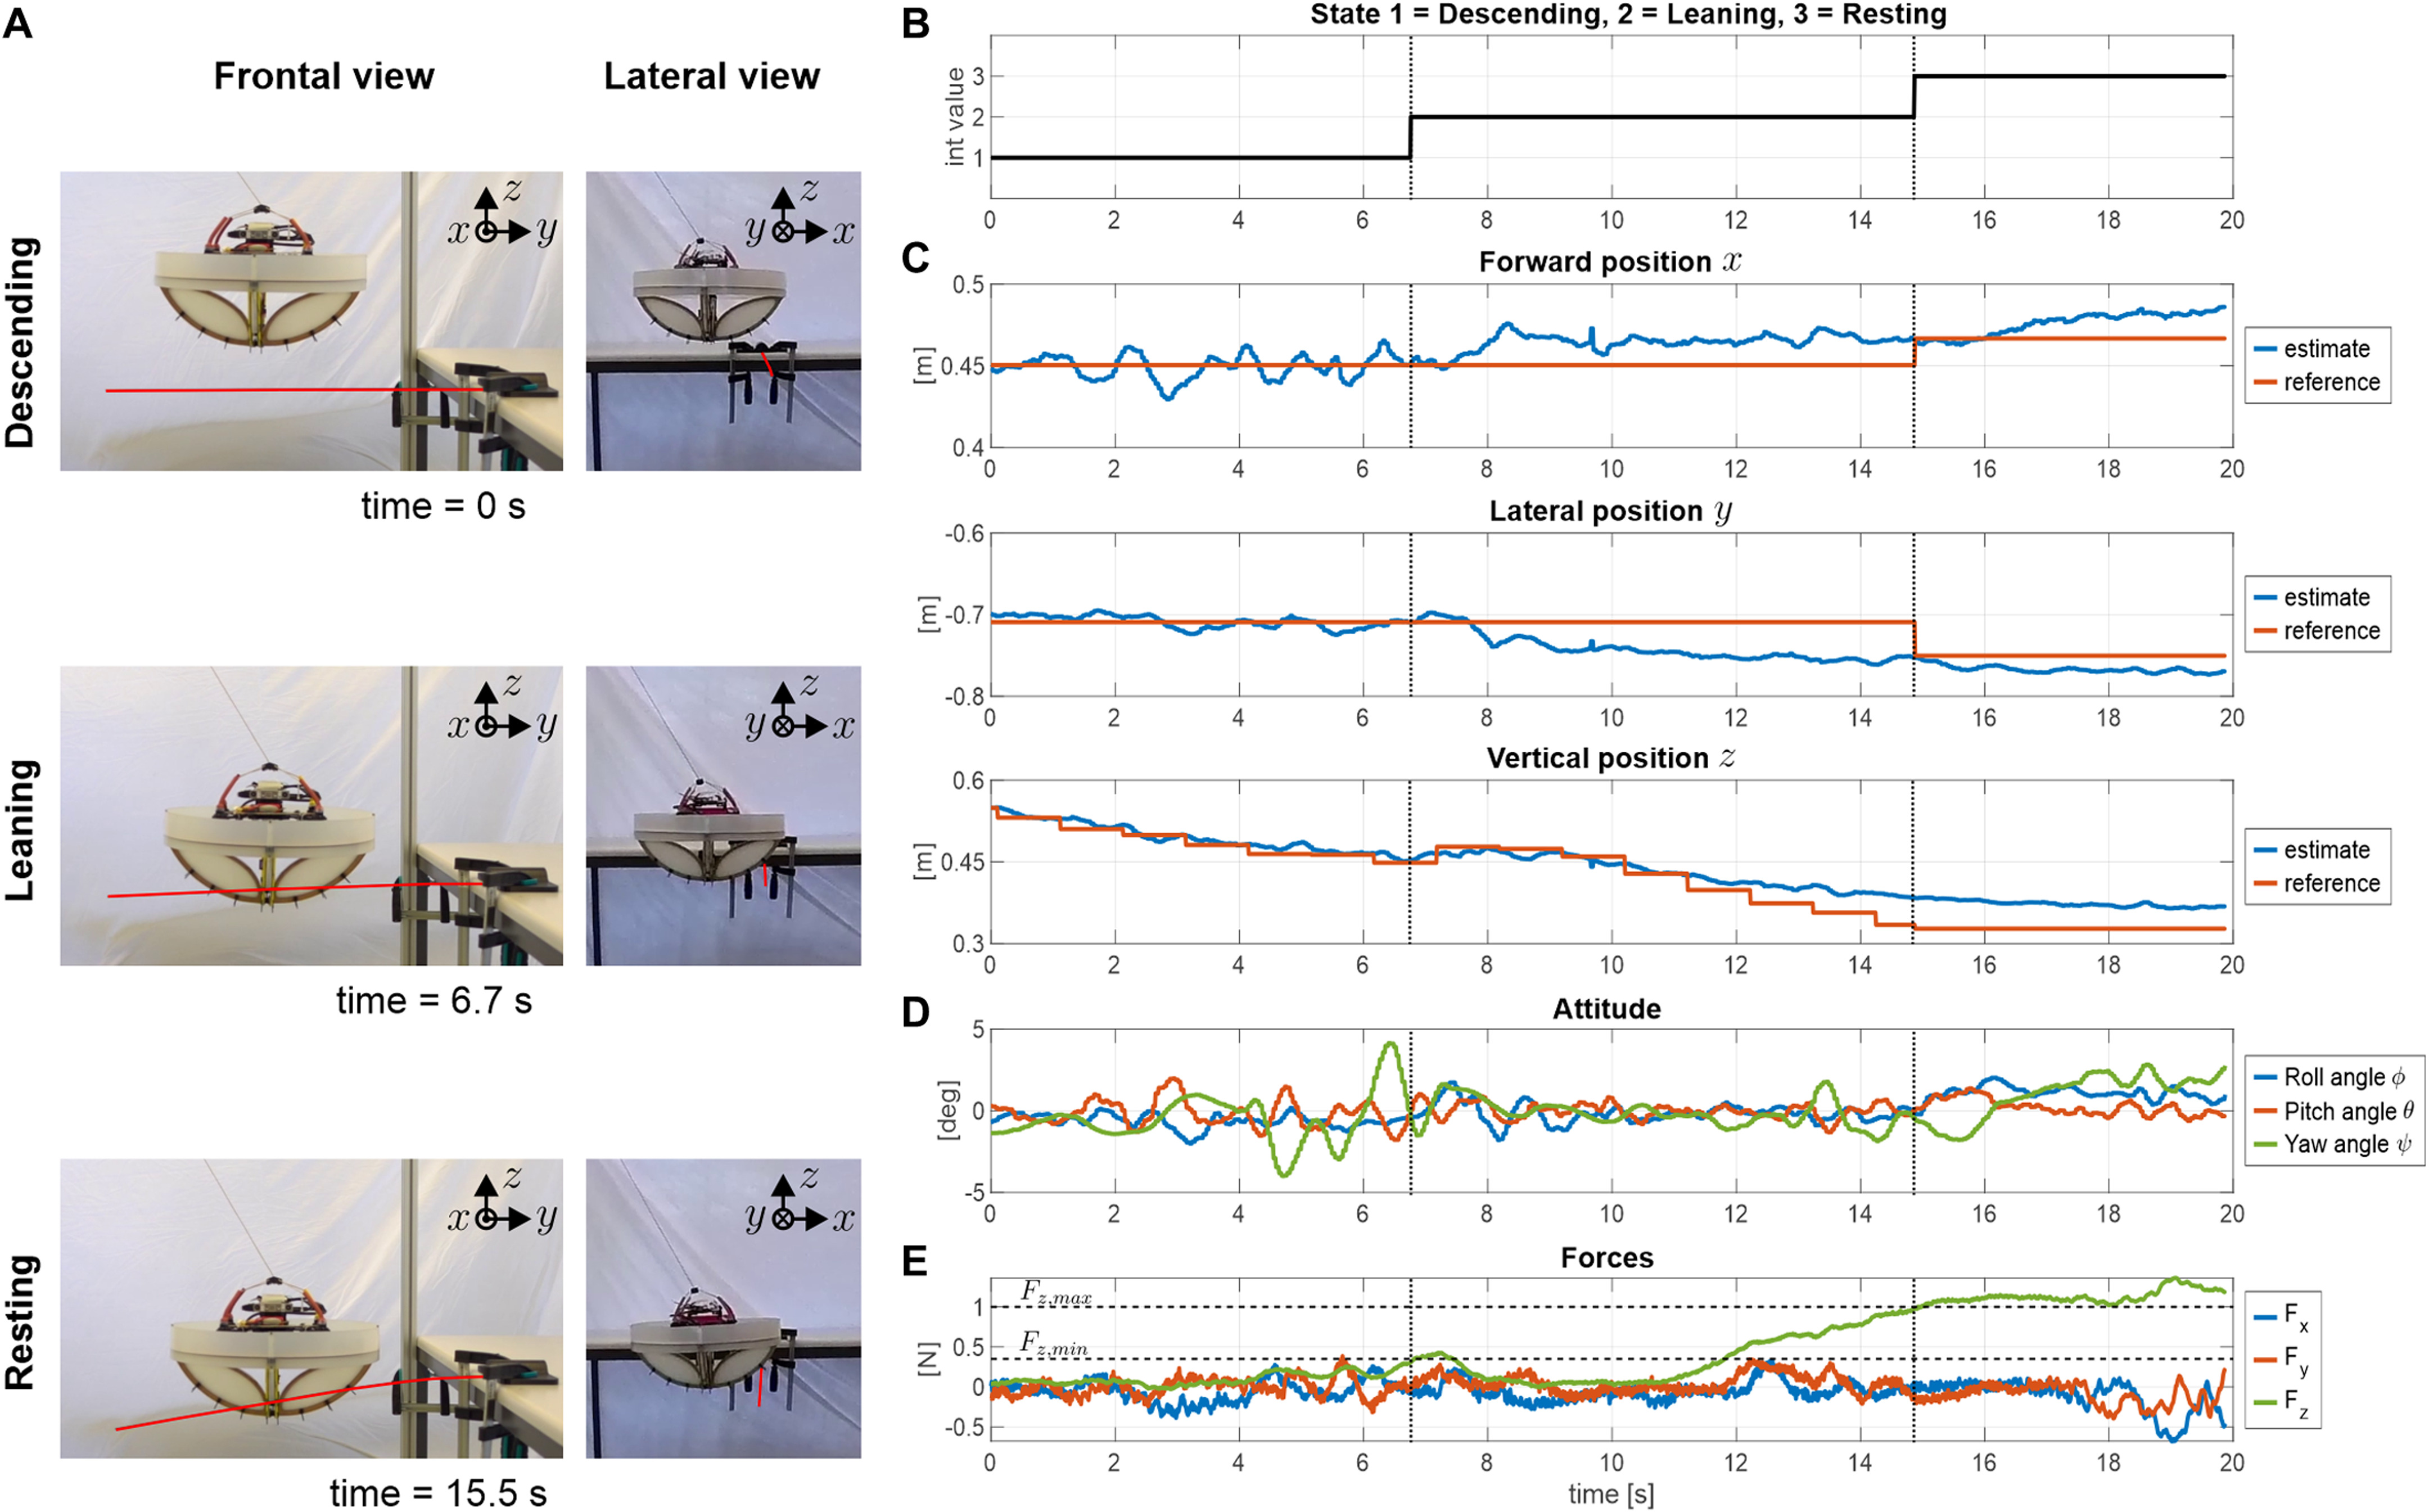
\includegraphics[scale = 0.9]{hinh 4}
    \caption{\textit{Thí nghiệm hạ cánh trên xà dẻo ($K = 1$  N/m)}}
    \label{fig4}
\end{figure}
Chúng tôi đã đánh giá độ bền và tính linh hoạt của chiến lược hạ cánh thông qua 110 lần hạ cánh trên các dầm đúc hẫng với các độ cứng khác nhau.
\newpage
\begin{figure}[ht!]
    \centering
    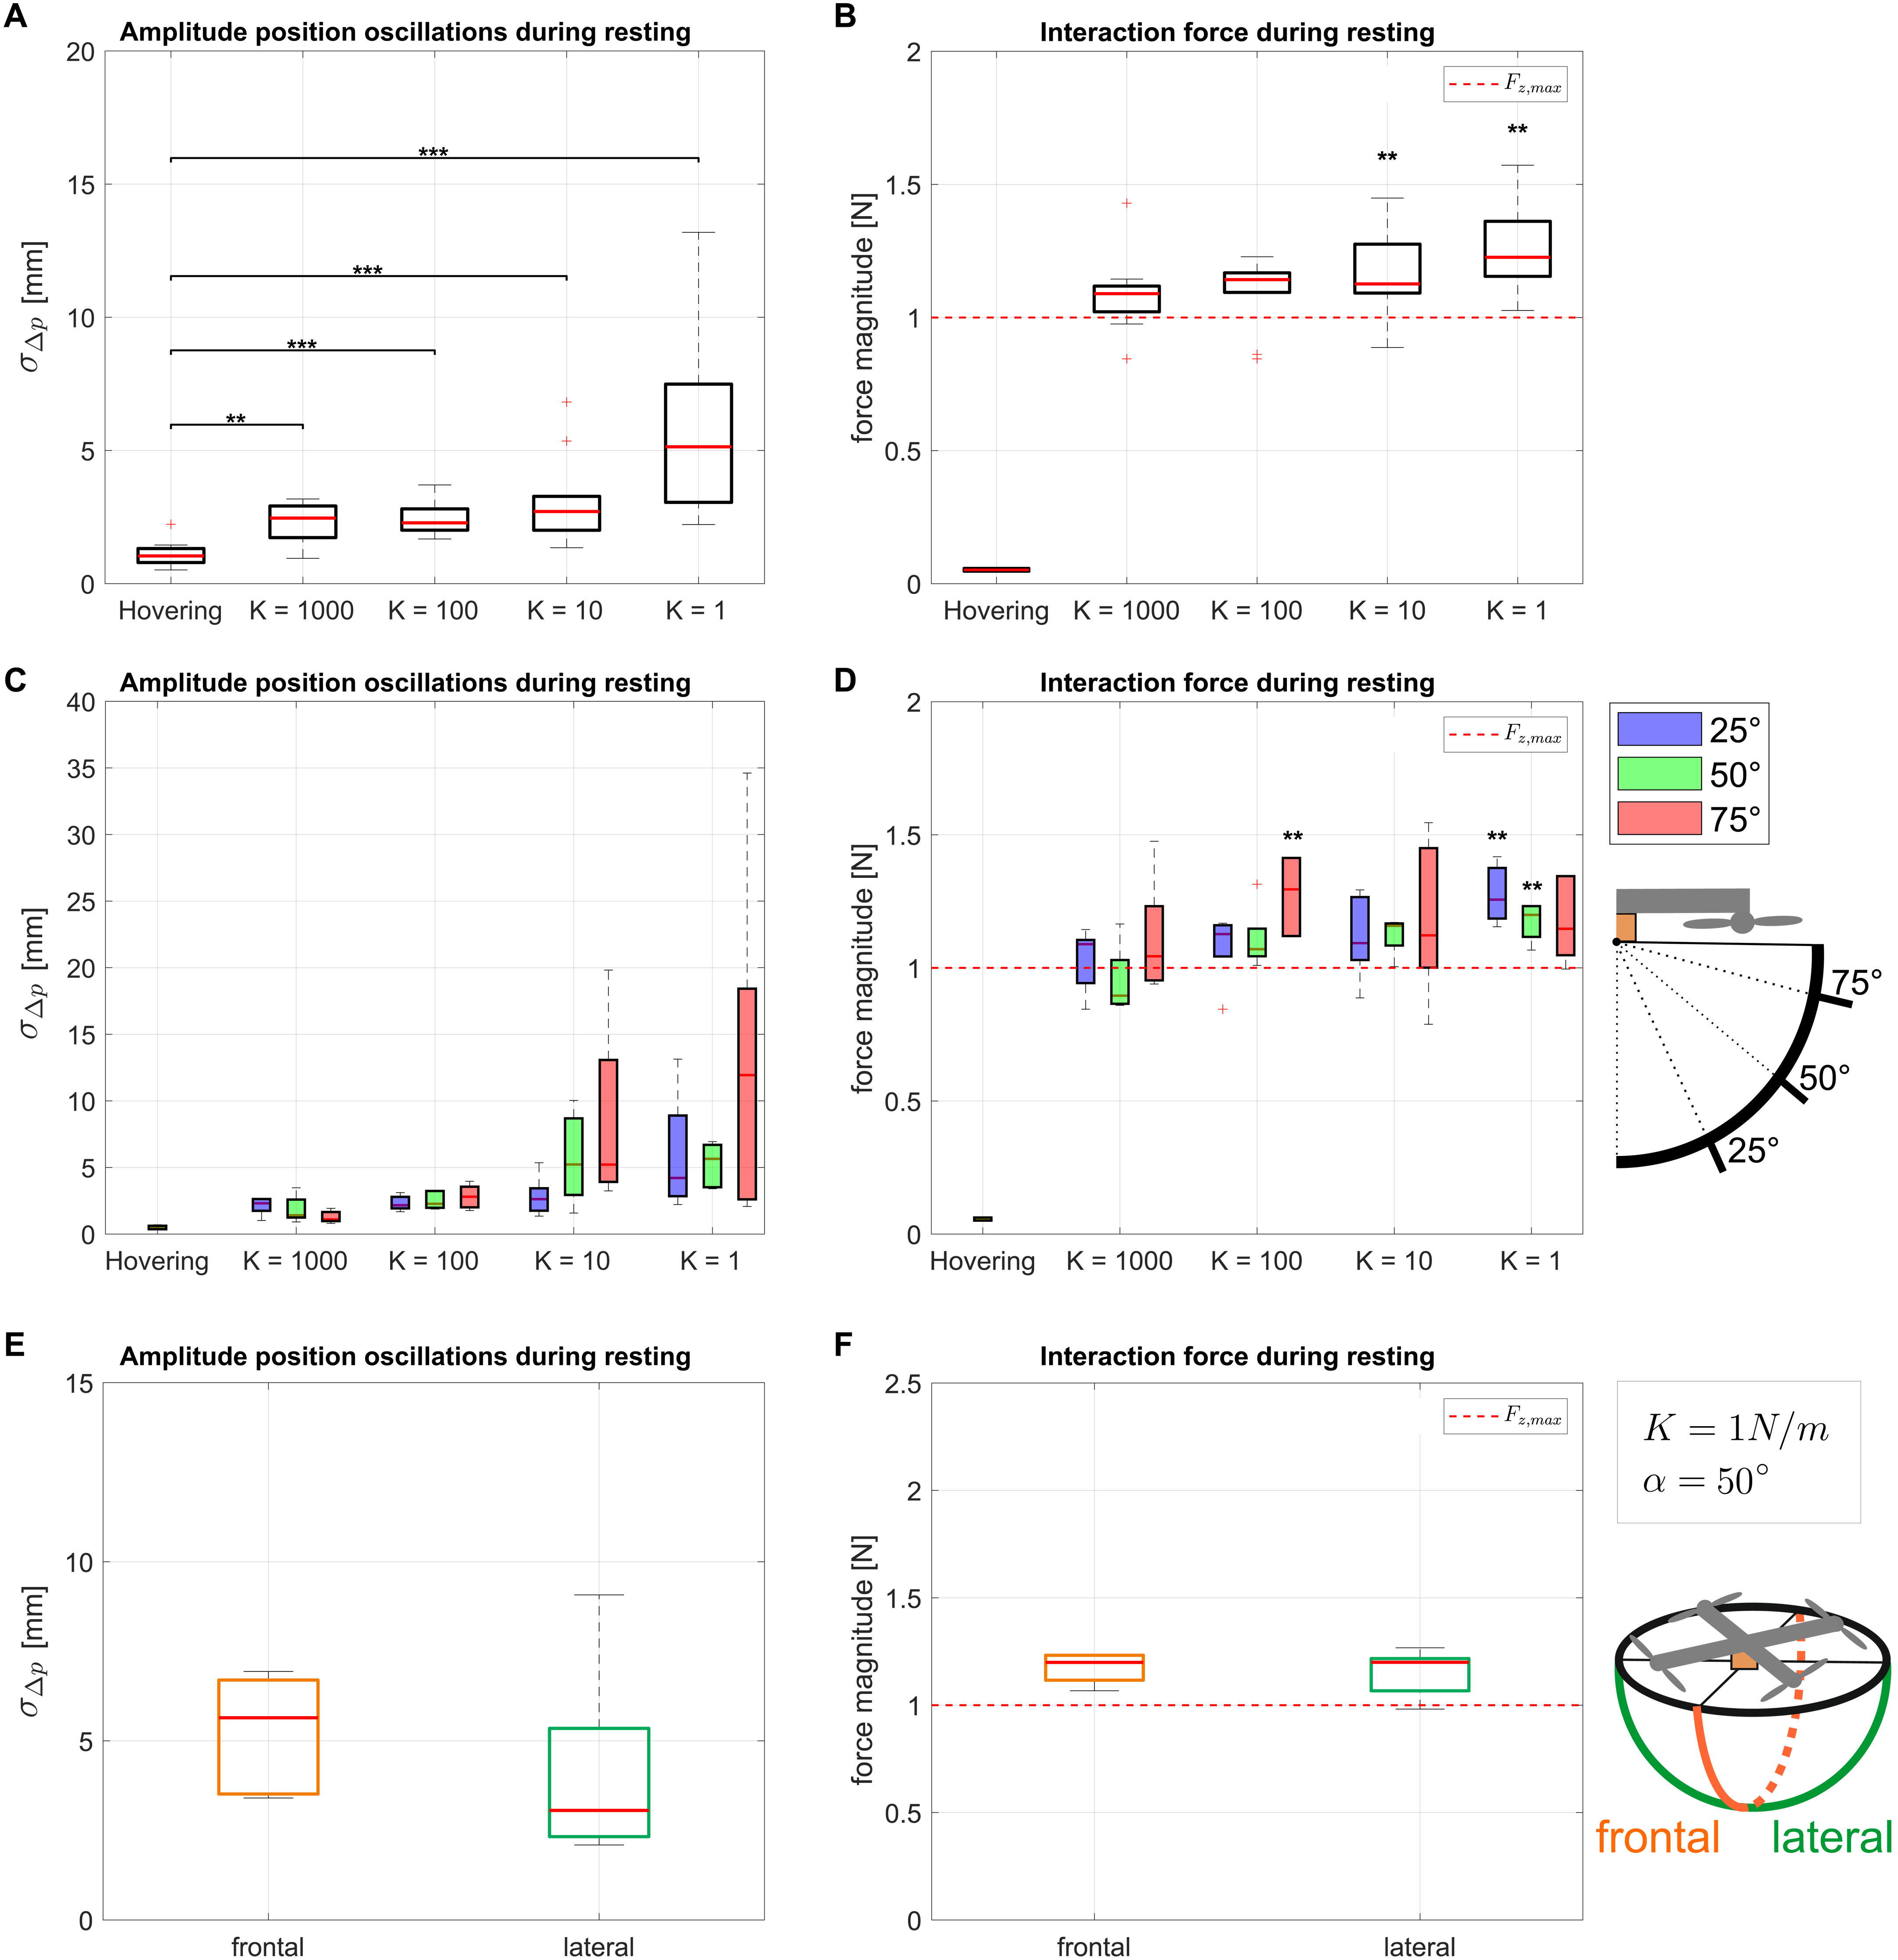
\includegraphics[scale = 0.6]{hinh 5}
    \caption{\textit{Xác thực thử nghiệm chiến lược tương tác.}}
    \label{fig5}
\end{figure}
\begin{figure}[ht!]
    \centering
    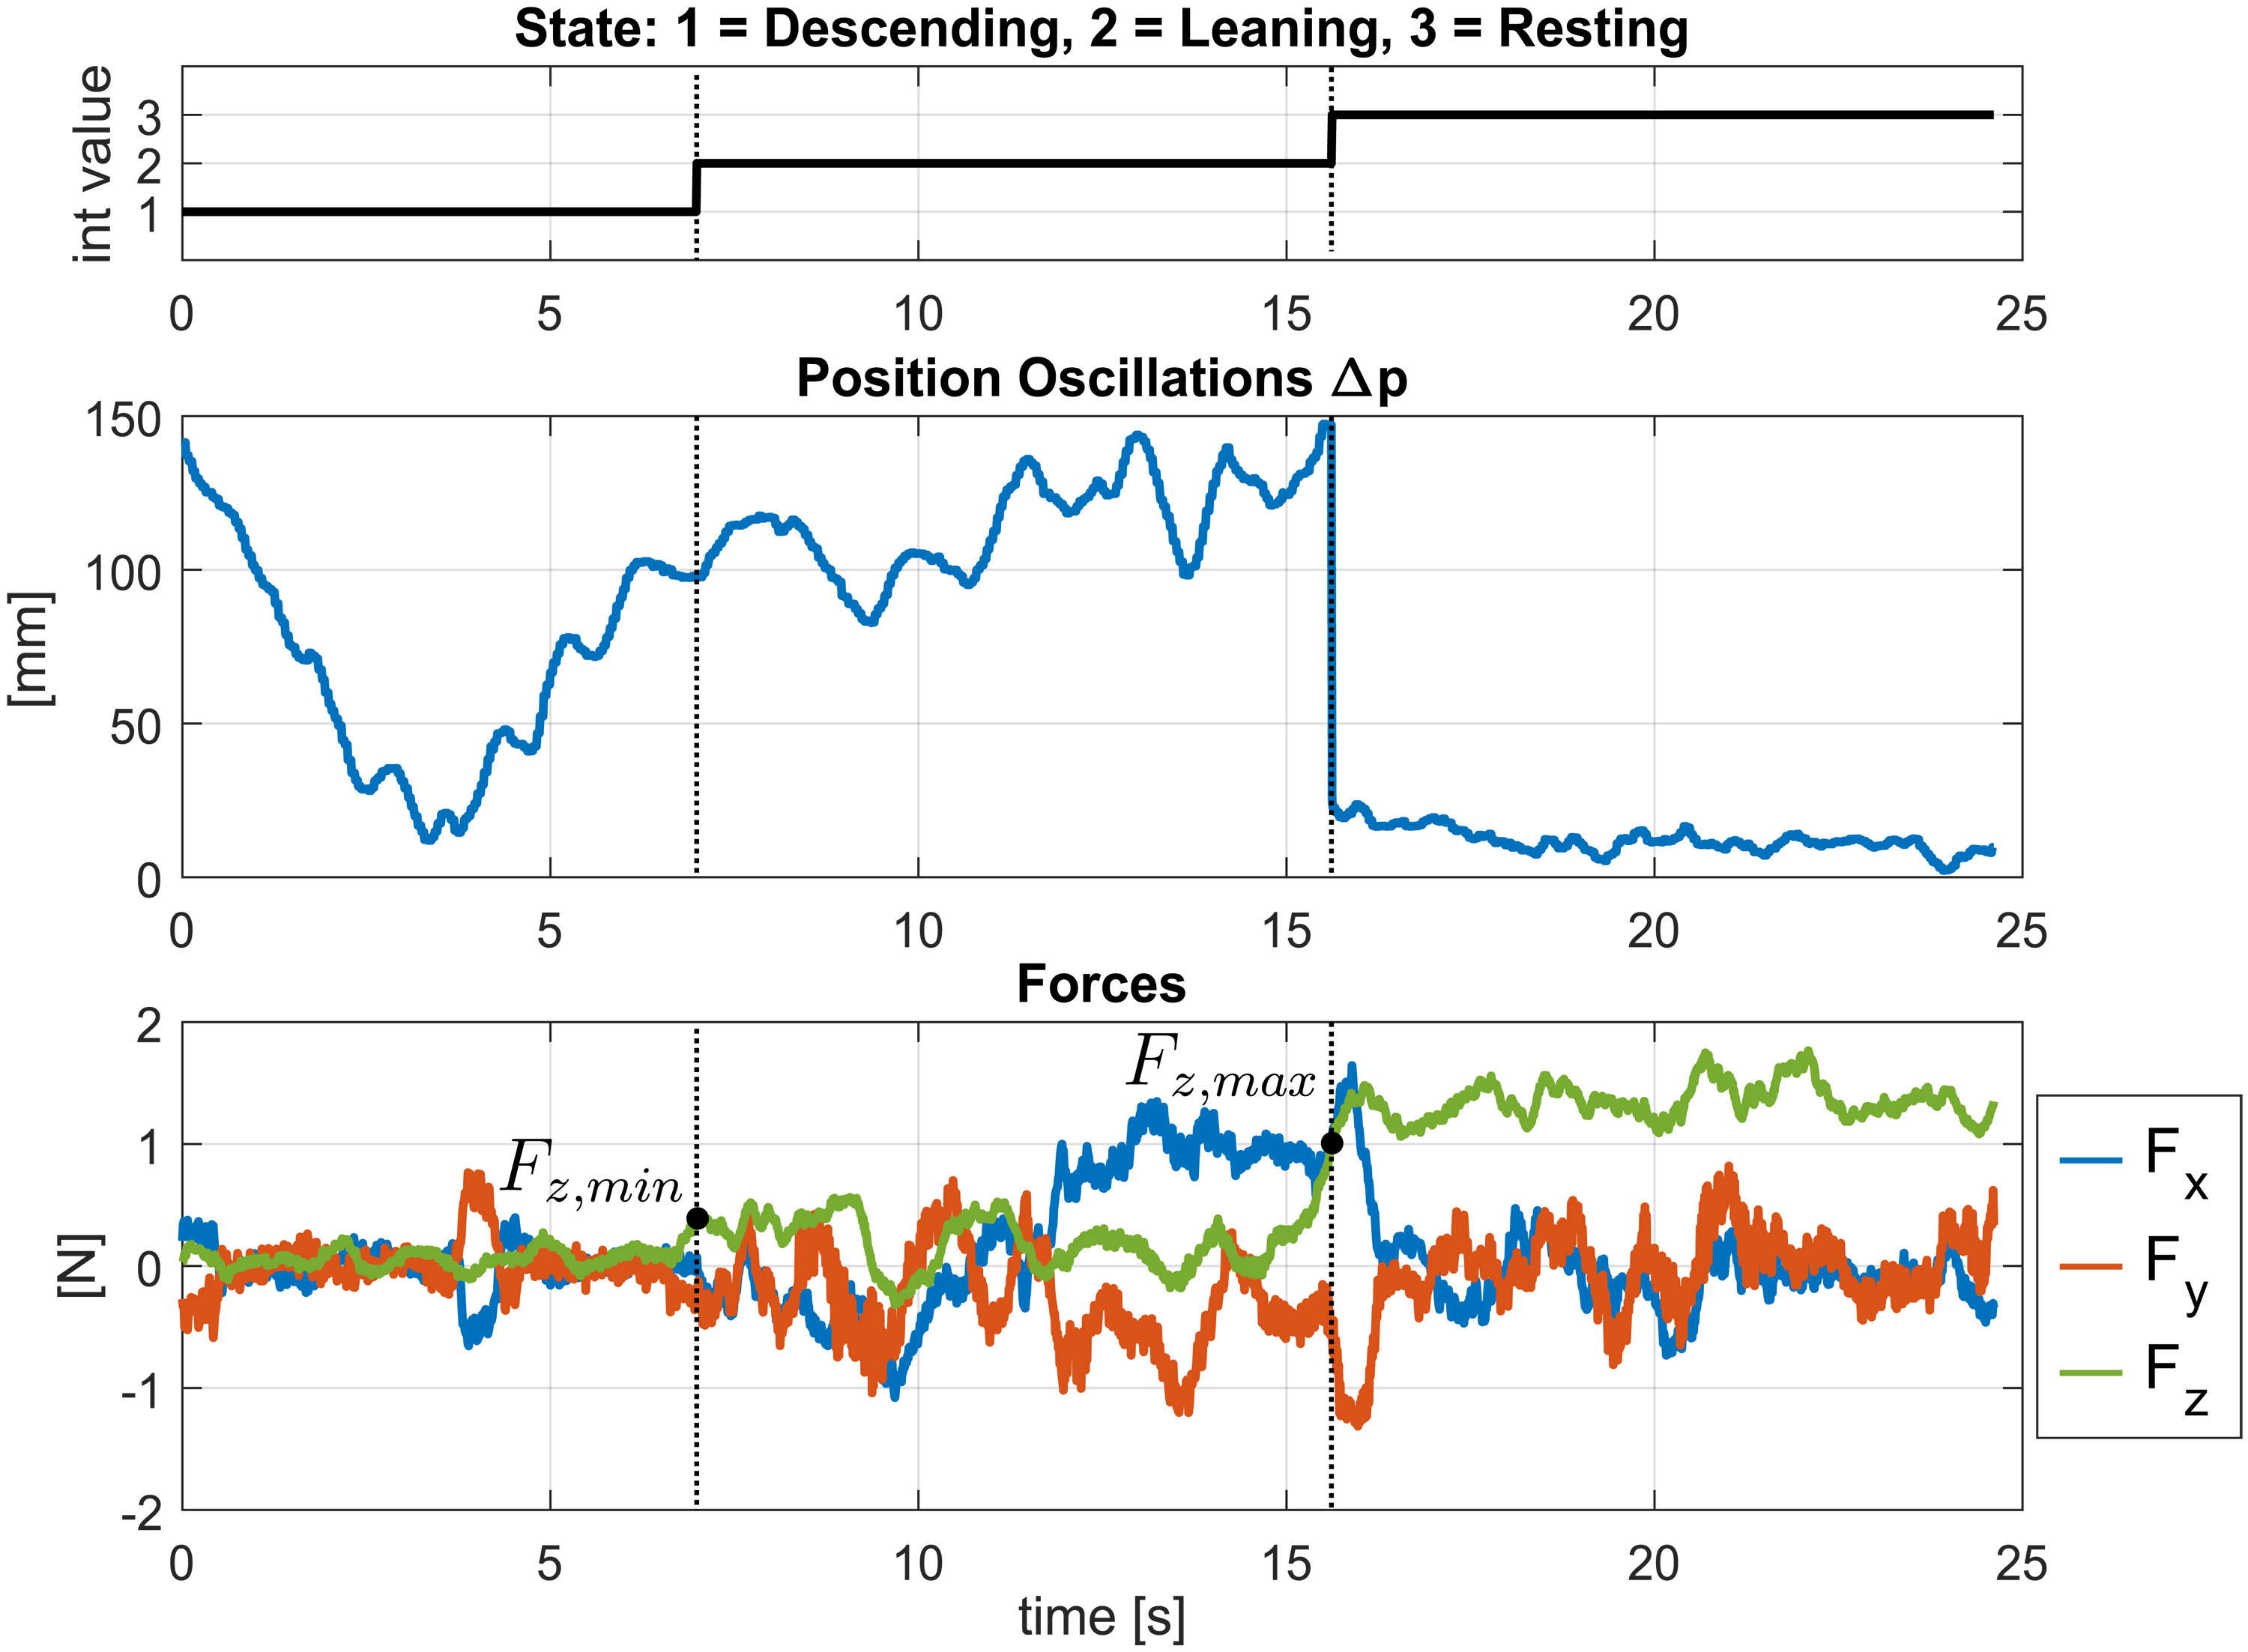
\includegraphics[scale = 0.6]{hinh 6}
    \caption{\textit{Ví dụ về kiểm tra ngoài trời.}}
    \label{fig6}
\end{figure}
\begin{center}
    \textbf{Kết quả trong thực nghiệm được thể hiện trên hình trên.}
\end{center}
\newpage
\subsection{Khảo Sát eDNA Bằng Chứng Về Khái Niệm}
Sau khi eDrone tiếp xúc với nhánh, eDNA bề mặt được thu thập bằng một bề mặt dính gắn vào các nắp của lồng. Chúng tôi quyết định chọn những loài cây khác nhau này, cả thực vật hạt kín và thực vật hạt trần, để kiểm tra tính hiệu quả của chiến lược hạ cánh trên các cành có hình thái khác nhau. Vì lý do an toàn, các điểm lấy mẫu được chọn trên các nhánh biệt lập để tránh va chạm không mong muốn với thảm thực vật trong giai đoạn tiếp cận.\\
\linebreak
Chúng tôi đã xác định được 21 loài với ưu thế là côn trùng nhưng cũng có một số động vật có xương sống như động vật có vú, chim và lưỡng cư. Chúng tôi đã quan sát thấy sự khác biệt trong việc phát hiện eDNA giữa các ngày lấy mẫu. Cụ thể, khi bắt đầu thí nghiệm, tất cả các mẫu đều thu được eDNA của các loài động vật (nghĩa là cả hai vật liệu đều hoạt động), bao gồm 10 loài động vật chân đốt và 5 loài có xương sống. Trong phần cuối cùng của thí nghiệm, chúng tôi chỉ xác định được một số loài (bao gồm bảy loài côn trùng mới và một loài động vật có vú), và vào ngày cuối cùng, chỉ có dấu vết DNA trên tấm gạc.\\
\begin{figure}[ht!]
    \centering
    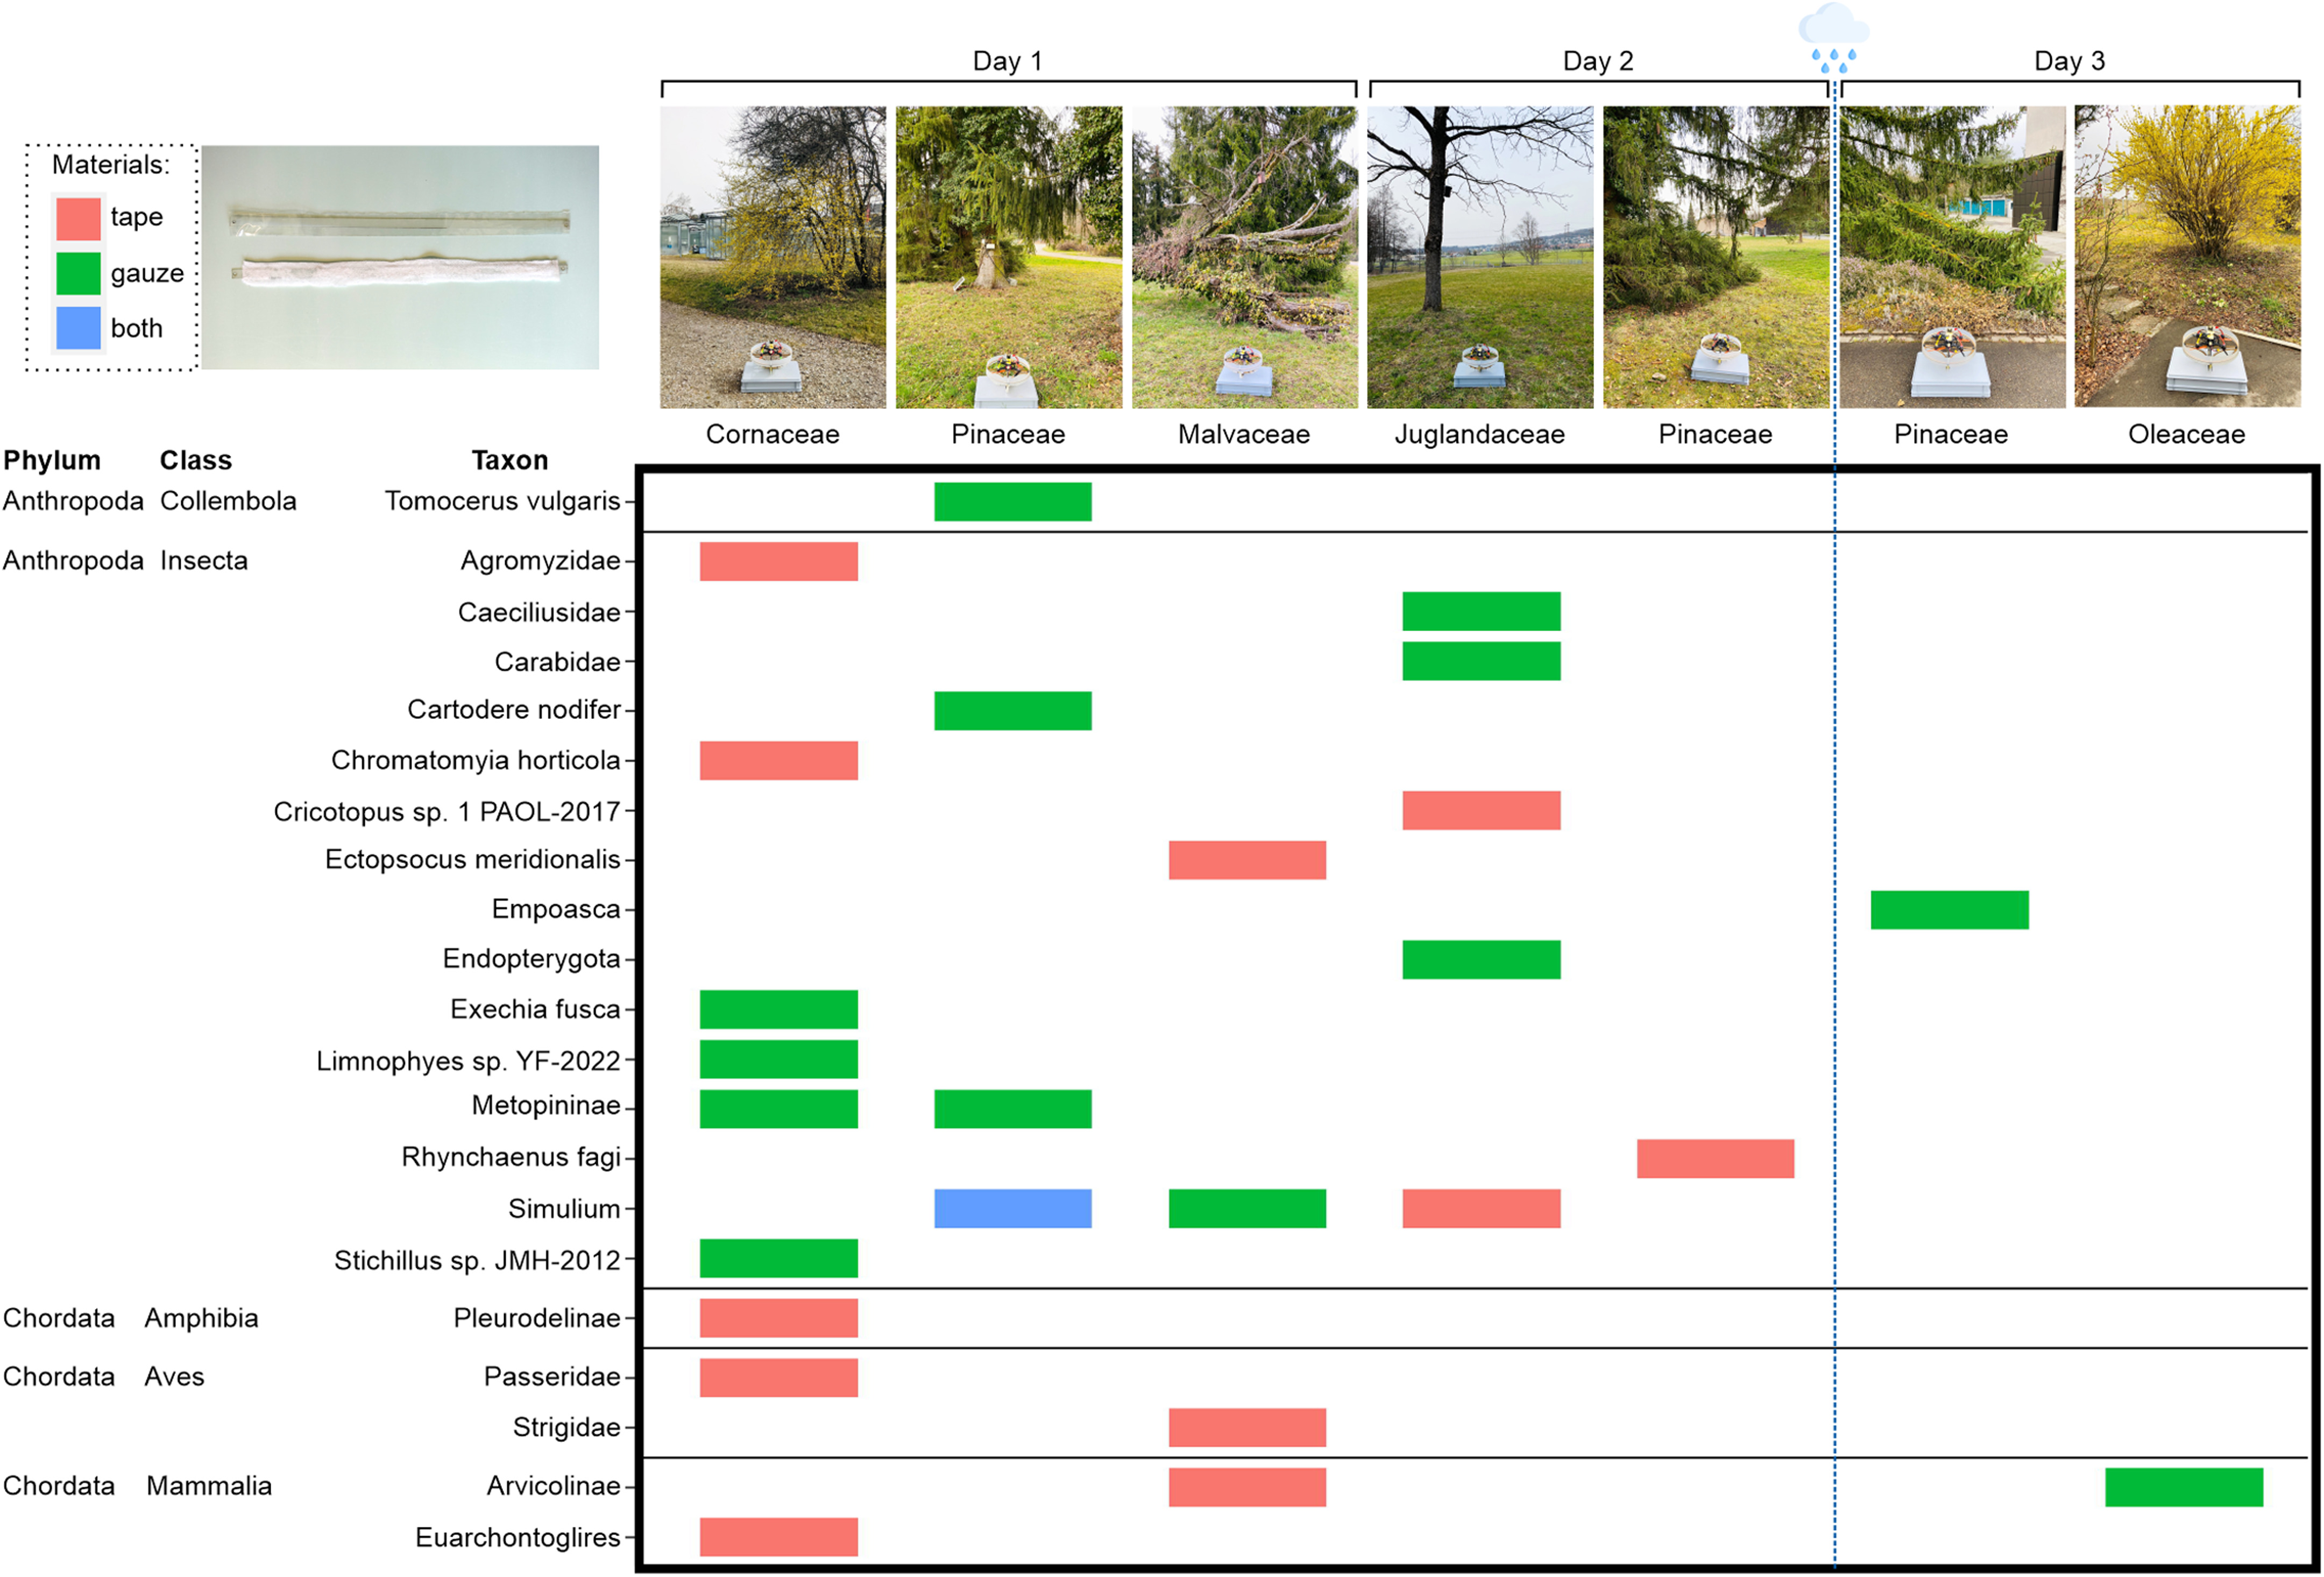
\includegraphics[scale = 0.7]{hinh 7}
    \caption{\textit{Các thí nghiệm lấy mẫu eDNA báo cáo các loài được phát hiện (ngành, lớp và đơn vị phân loại) liên quan đến các vật liệu thu thập cụ thể và các loài cây.}}
    \label{fig7}
\end{figure}
\newpage
\section{Vật Liệu Và Phương Pháp}
\subsection{Vật Liệu Làm Máy Bay}
eDrone đã sử dụng bố cục quadcopter bao gồm khung bằng sợi carbon và bốn động cơ không chổi than (Dys THOR 2408, 2200KV) với cánh quạt 6 inch (Gemfan 6040) được điều khiển bởi bộ điều khiển tốc độ điện tử (Hobbywing XRotor 40A 4in1 ESC). Bộ điều khiển chuyến bay ổn định tư thế của máy bay không người lái (BrainFPV, Radix LI). Camera theo dõi Intel RealSense T261 cung cấp ước tính quán tính trực quan và máy tính đồng hành Khadas VIM3 cung cấp bộ điều khiển vị trí cấp cao, giao tiếp không dây và tính toán bổ sung trên máy bay. Ngoại lực do nhánh tác dụng lên máy bay không người lái được đo bằng cảm biến Medusa F/T (Bota Systems AG, Thụy Sĩ).\\
\subsection{Sản Xuất Lồng}
Các liên kết chính của lồng, vòng ngang và các vòng cung dọc được cắt bằng laze (Trotec Speedy 360) từ các tấm ván sợi mật độ trung bình 3 mm. Các thành phần được kết nối thông qua các thành phần in 3D (Stratasys F120) và được cố định bằng vít. Các nắp bộ sưu tập được làm bằng sợi thủy tinh (FR-40-HF, 0,2 mm) và được kết nối với lồng bằng vít. Lồng được thiết kế sao cho có thể mở đồng thời bốn nắp bộ sưu tập để lấy mẫu. Vòng tròn bên ngoài được thêm vào để che chắn các cánh quạt cũng được làm bằng sợi thủy tinh. Các thanh công xôn được chế tạo bằng dầm carbon 2 mm và vật liệu có độ ma sát cao là Dycem nonslip.\\
\subsection{Kiến Trúc Điều Khiển }
Kiến trúc điều khiển và cảm biến hoàn chỉnh của eDrone được mô tả trong hình dưới đây. Cảm biến lực đo ngoại lực trong khung thân, do đó HWR đã chuyển đổi nó thành khung thế giới bằng cách sử dụng hướng của khung cơ thể đối với khung thế giới, dẫn đến ngoại lực cho toàn bộ hệ thống. Bộ điều khiển này có thể nhận tham chiếu và độ lệch. Trong giai đoạn đi xuống và đi nghiêng, HWR đã gửi các điểm tham chiếu dọc $\textit{p}_{ref} = [x, y, z -\Delta{z}]$, trong giai đoạn nghỉ nó khai thác thông tin về biên độ và hướng của lực bằng cách ra lệnh cho một điểm tham chiếu 3D, theo phương trình\\
 $$P_{resting} = P_{ref} = P - C_{gain} \frac{F_{ext}}{\|{F_{ext}}\|} $$ \\
 Trong đó $C_{gain}$ là mức tăng của bộ điều khiển có thể được điều chỉnh tùy thuộc vào lực chúng ta muốn tác dụng lên nhánh.\\
 \begin{figure}[ht!]
    \centering
    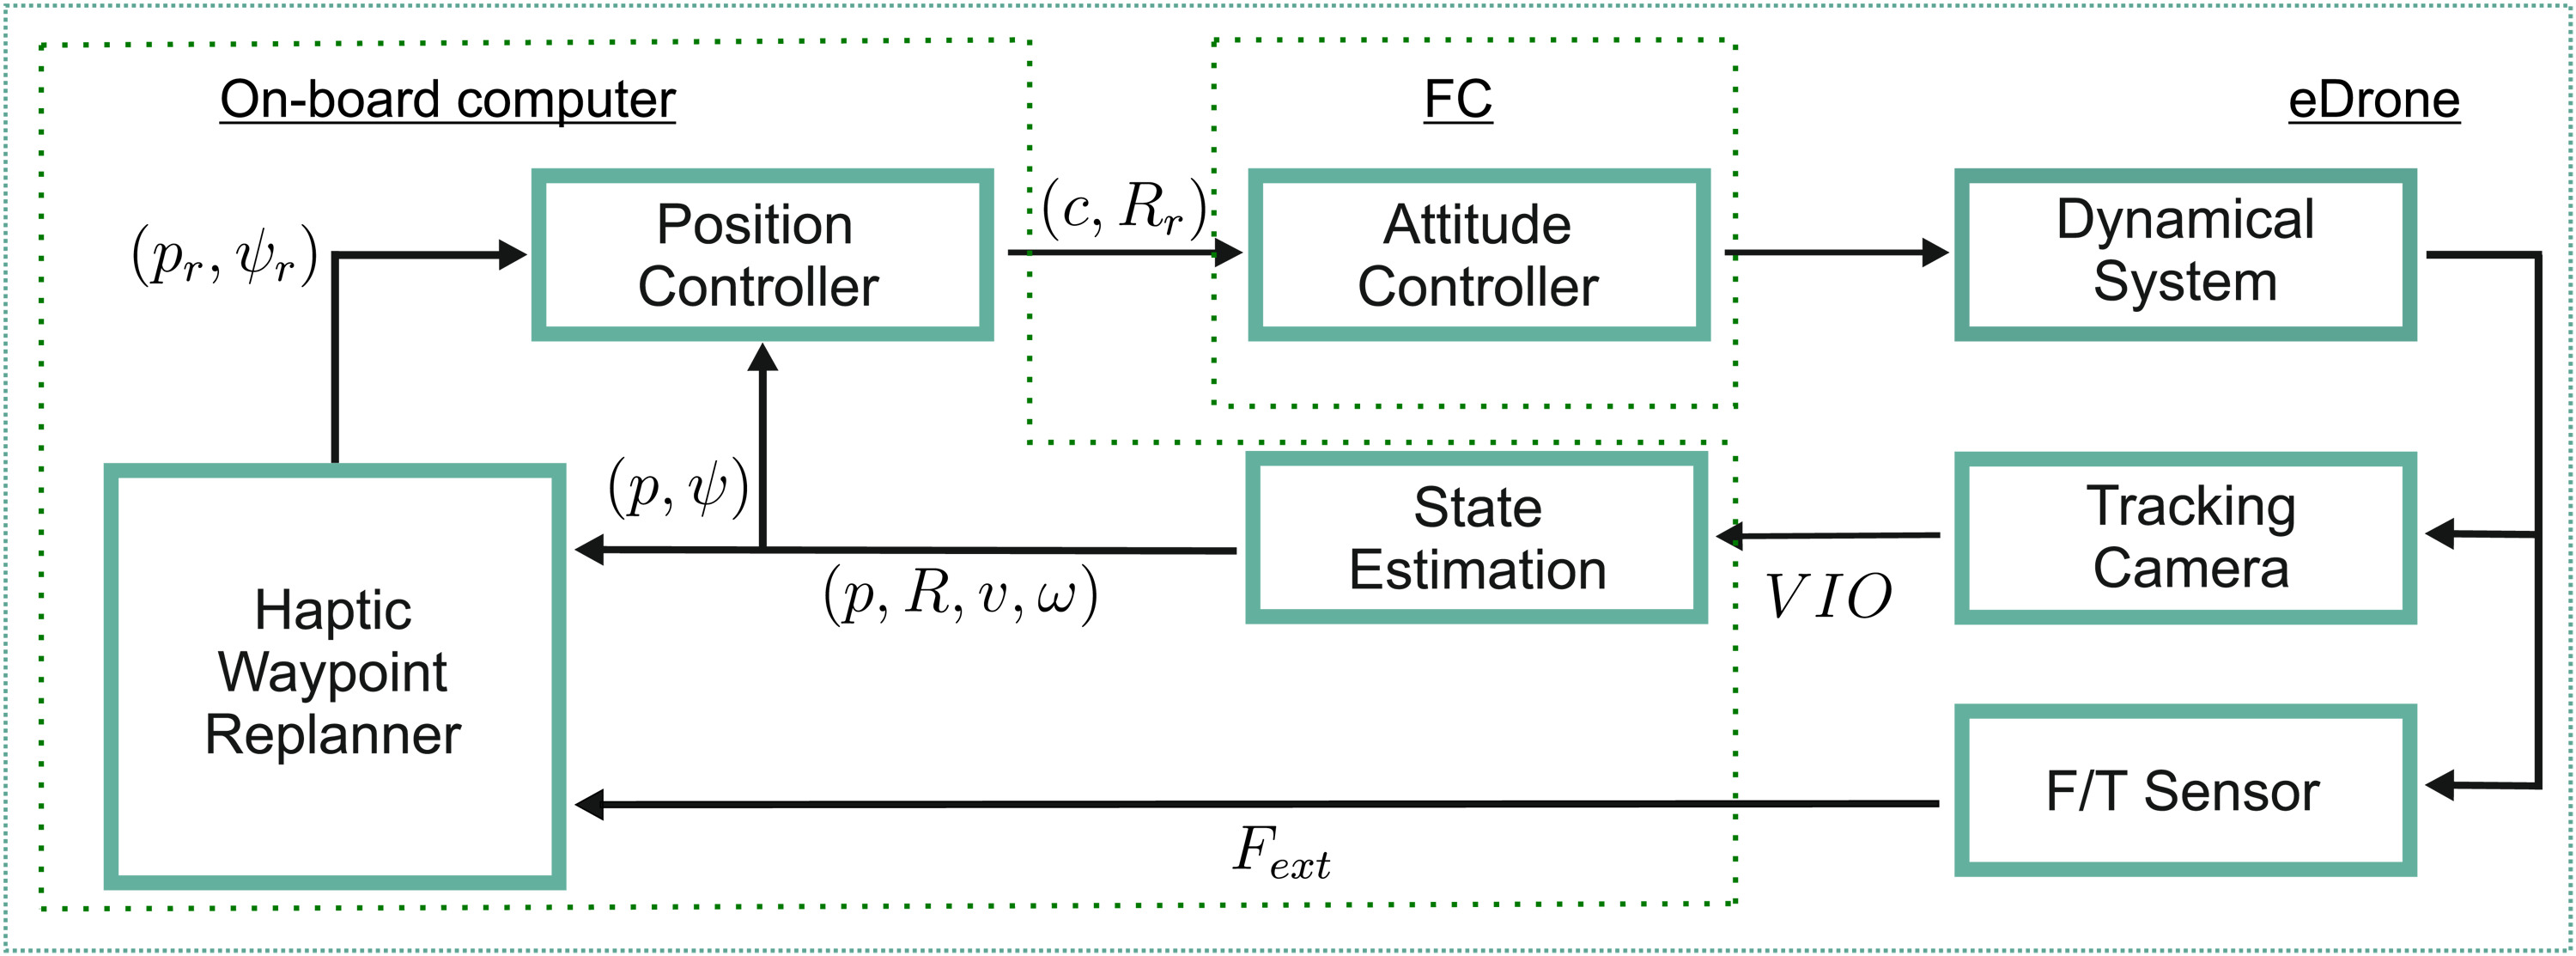
\includegraphics[scale = 1]{hinh 8}
    \caption{\textit{Sơ đồ khối của các thành phần hệ thống và kiến trúc điều khiển.}}
    \label{fig8}
\end{figure}
\subsection{Phân Tích Thống Kê}
Để có được sự phân phối dữ liệu mà chúng tôi đã sử dụng để phân tích thống kê hiệu suất cho các độ cứng và độ chênh lệch khác nhau giữa các máy bay không người lái, chúng tôi đã chính xuất một giá trị SD của lỗi vị trí và lực tương tác trung bình khi xem xét khoảng thời gian của giai đoạn nghỉ ngơi cho mỗi thử nghiệm hạ cánh. Do đó, khi thử nghiệm N, chúng tôi đã có một phân phối bao gồm các giá trị N. Thử nghiệm Mann-Whitney U được thực hiện trong MATLAB R2020a.\\
\subsection{Tài Liệu Thu Thập eDNA}
Do khó khăn trong việc lấy mẫu eDNA từ cây nên tài liệu về các vật liệu để lấy dấu vết eDNA từ vỏ cành cây còn hạn chế. Lấy cảm hứng từ kỹ thuật bóc tách được khai thác trong các cuộc điều tra pháp y, chúng tôi đã sử dụng băng dính vô trùng vì băng dính này có thể dễ dàng ấn vào các bề mặt và lấy ra các hạt chứa eDNA. Nước tạo điều kiện thuận lợi cho việc chuyển eDNA từ chất nền khô, trong khi đường bổ sung tác dụng kết dính chất thu gom. Chúng tôi đã chọn một miếng gạc bông đàn hồi đã khử trùng và làm ẩm nó bằng dung dịch tự nhiên, được khuấy và bảo quản trong các ống vô trùng 10ml.\\
\subsection{Phân Tích eDNA}
Trích xuất DNA được thực hiện theo một giao thức đã sửa đổi từ trong phòng thí nghiệm eDNA chuyên dụng được trang bị áp suất không khí dương, xử lý tia cực tím và đổi mới không khí thường xuyên. Các thủ tục khử nhiễm được tiến hành trước và sau tất cả các thao tác. Các mẫu được phân tích bằng cách sử dụng metazoan. Khi chọn một điểm đánh dấu mã hóa siêu dữ liệu, luôn có sự đánh đổi giữa tính phổ biến của đoạn mồi và độ phân giải của đoạn được khuếch đại. Tuy nhiên, khi sử dụng những dấu hiệu phổ biến như vậy có thể phát hiện nhiều nhóm phân loại khác nhau, nhưng sự biến đổi trình tự không cho phép xác định cấp độ loài, như được phản ánh ở kết quả phân tích. Các sản phẩm PCR tinh khiết được gộp lại trước các bước giải trình tự với các thể tích bằng nhau để đạt được độ sâu giải trình tự theo lý thuyết là 100.000 lượt đọc trên mỗi mẫu. Quá trình khuếch đại và tinh sạch PCR được thực hiện trong phòng dành riêng cho phân tích DNA khuếch đại với áp suất không khí âm và được tách biệt về mặt vật lý với phòng chiết tách eDNA. \\
\section{Kết Quả}
Drones thể hiện tiềm năng khai thác robot để giám sát đa dạng sinh học bằng cách lấy mẫu thành công eDNA từ cành cây. Máy bay không người lái được điều khiển từ xa qua một nhánh bằng cách sử dụng phản hồi trực quan từ camera trên máy bay. Khi gần đạt được sự liên kết mong muốn, máy bay không người lái tự động hạ cánh và nằm trên cành cây. Trong thời gian này, bộ thu eDNA ở bề mặt ngoài cùng của lồng chạm vào vỏ cây để lấy eDNA bề mặt. Sau đó, eDrone quay trở lại di chuột phía trên nhánh và được điều khiển từ xa trở lại khu vực hạ cánh được chỉ định, nơi các bộ sưu tập eDNA được gỡ bỏ và lưu trữ. Sau đó, các mẫu được xử lý theo quy trình mã hóa siêu dữ liệu eDNA cho khảo sát đa dạng sinh học. Các thí nghiệm thực địa đã dẫn đến việc xác định được 21 đơn vị phân loại khác nhau.\\
\section{Tài Liệu Tham Khảo}
\begin{thebibliography}{9}
\bibitem{book}
IPBES, \textit{Global Assessment Report on Biodiversity and Ecosystem Services of the Intergovernmental Science-Policy Platform on Biodiversity and Ecosystem Services }(2019),10.5281/zenodo.3831673.
\newpage
\bibitem{book}
M.Loreau, S.Naeem, P.Inchausti, J.Bengtsson, J.P.Grime, A.Hector, D.U.Hooper, M.A.Huston, D.Raffaelli, B.Schmid, D.Tilman, D.A.Wardle, Biodiversity and ecosystem functioning: Current knowledge and future challenges. \textit{Science} 294, 804 - 808 (2001).\\
\bibitem{book}
B.J.Cardinale, J.E.Duffy, A.Gonzalez, D.U.Hooper, C.Perrings, P.Venail, A. Narwani, G.M.MacE, D.Tilman, D.A.Wardle, A.P.Kinzig, G.C.Daily, M.Loreau, J.B.Grace, A.Larigauderie, D.S.Srivastava, S.Naeem, Biodiversity loss and its impact on humanity. \textit{Nature} 486, 59–67 (2012).
\end{thebibliography}
\end{document}